\documentclass[a4paper,12pt,Times]{article}
\usepackage{abakos}  %pacote com padrão da Abakos baseado no padrão da PUC
\usepackage{forest}
%%%%%%%%%%%%%%%%%%%%%%%%%%%
%Capa da revista
%%%%%%%%%%%%%%%%%%%%%%%%%%

%\setcounter{page}{80} %iniciar contador de pagina de valor especificado
\newcommand{\monog}{Trabalho Prático de Algoritmos e Estrutura de Dados III - Entrega 2}
\newcommand{\monogES}{Model - Magazine Abakós - ICEI - PUC Minas}
\newcommand{\tipo}{Artigo }  % Especificar a seção tipo do trabalho: Artigo, Resumo, Tese, Dociê etc
\newcommand{\origem}{Brasil}
\newcommand{\editorial}{\textbf{Abakos}, Belo Horizonte,v. 1, n. 1, p. 00-00, Ago. 2021 - ISSN: 2316-9451}  % p. xx-xx – páginas inicial-final do artigo
% \newcommand{\lcc}{\scriptsize{Licença Creative Commons Attribution-NonCommercial-NoDerivs 3.0 Unported}}

%%%%%%%%%%%%%%%%%INFORMAÇÕES SOBRE AUTOR PRINCIPAL %%%%%%%%%%%%%%%%%%%%%%%%%%%%%%%
\newcommand{\AutorA}{Henrique Castro e Silva}
\newcommand{\funcaoA}{}
\newcommand{\emailA}{henrique.silva.1281914@pucminas.br}
\newcommand{\cursA}{Programa de Graduação em Ciência da computação da PUC Minas}

\newcommand{\AutorB}{Leonardo Caetano Gomide}
\newcommand{\funcaoB}{}
\newcommand{\emailB}{lcgomide@sga.pucminas.br}
\newcommand{\cursB}{Programa de Graduação em Ciência da computação da PUC Minas}

% Definir macros para o nome da Instituição, da Faculdade, etc.
\newcommand{\univ}{Pontifícia Universidade Católica de Minas Gerais}

\newcommand{\keyword}[1]{\textsf{#1}}

\begin{document}
% %%%%%%%%%%%%%%%%%%%%%%%%%%%%%%%%%%
% %% Pagina de titulo
% %%%%%%%%%%%%%%%%%%%%%%%%%%%%%%%%%%

\begin{flushleft}

\begin{minipage} [c][3cm][b]{15cm} % a primeira minipágina tem uma altura de 1.5cm e uma largura de 2.3cm.
% comando que introduz o logo da escola que nesta altura já terá de estar na pasta imagens que 
%por sua vez está na pasta onde se guardou o arquivo tex. E introduzimos essa imagem com a mesma altura da minipage.
\begin{flushleft}

\includegraphics[scale=1.5]{figuras/header.png} 
\end{flushleft}
\end{minipage}

 \vspace{0cm} {
 \singlespacing \Large{\monog \\ }
  \normalsize{\monogES}
 }
\end{flushleft}
\begin{flushright}
\singlespacing 
\normalsize{\AutorA \footnote{\funcaoA \cursA, \origem -- \emailA }} \\
\normalsize{\AutorB \footnote{\funcaoB \cursB, \origem -- \emailB }} \\
% \normalsize{\AutorC \footnote{\funcaoC, E-mail:\emailC \\ \cursC, \origem. }} \\
% \normalsize{\AutorD \footnote{\funcaoD \\ Pais de origem: \origemD. E-mail: \emailD}} \\
%deixar com o valor `0` e usar o '*' no inicio da frase
% \symbolfootnote[0]{Artigo recebido em 10 de julho de 1983 e aprovado em 29 de maio 2012}
\end{flushright}
\thispagestyle{empty}

\begin{abstract}
\noindent
Este trabalho tem como intenção desenvolver um sistema que faça manipulação de arquivos em memória primária e secundária. O sistema em questão, consiste em um cadastro de prontuários para um empresas de planos de saúde, com opções de inserção, alteração, exclusão e impressão. Conforme estipulado pelo cronograma da disciplina, este trabalho será composto por três entregas complementares, cada entrega responsável por entregar diferentes artefatos. Este documento é referente à primeira entrega, que é composta por diferentes artefatos que foram desenvolvidos pelos alunos. Esses artefatos incluem a criação de um arquivo mestre, o desenvolvimento de um sistema que faça todas as operações de CRUD (criar, ler, atualizar e deletar) e produção de um documento de texto. Para o desenvolvimento dos diferentes requisitos técnicos foram desenvolvidas diferentes classes e funções. A formatação do arquivo mestre, a finalidade e as especificações de cada classe e o funcionamento do sistema em geral serão abordadas neste documento.
\\\textbf{\keyword{Palavras-chave: }} Algoritmos e Estrutura de Dados. CRUD. Manipulação de arquivos.
\end{abstract}

%%%%%%%%%%%%%%%%%%%%%%%%%%%%%%%%%%%%%%%%%%%%%%%%%%%%%%%%%
\newpage 
\selectlanguage{english}
\begin{abstract}
\noindent
This assignment focused on developing a system that may manipulate files in primary and secondary memory. The system consists of a registration of medical records, including insertion, updating, exclusion and printing options. According to the discipline’s stipulated schedule, this assignment will be composed of three complementary deliveries, each responsible to deliver different features. This document refers to the first delivery, which is composed by different features developed by the students. These features include the creation of a master file, a system’s development, which include all CRUD (create, read, update, delete) operations, and generation of textual document. In order to develop all the technical issues, different classes and functions were developed. The master file’s formatting, the purpose and specifications’ of each class and the overall systems’ running will be discussed in this document.
\\\textbf{\keyword{Keywords: }} Algorithms and Data Structure. CRUD. File manipulation.
\end{abstract}

\selectlanguage{brazilian}
 \onehalfspace  % espaçamento 1.5 entre linhas
 \setlength{\parindent}{1.25cm}

%%%%%%%%%%%%%%%%%%%%%%%%%%%%%%%%%%%%%%%%%%%%%%%%%
%% INICIO DO TEXTO
%%%%%%%%%%%%%%%%%%%%%%%%%%%%%%%%%%%%%%%%%%%%%%%%%

%%%%%%%%%%%%%%%%%%%%%%%%%%%%%%%%%%%%%%%%%%%%%%%%%%%%%%%%%%%%%%%%%%%%%%%%%%%%%%%%%%%%%%%%%%%%%%%%%%%%%%%
%%%%%%%%%%%%%% Template de Artigo Adaptado para Trabalho de Diplomação do ICEI %%%%%%%%%%%%%%%%%%%%%%%%
%% codificação UTF-8 - Abntex - Latex -  							     %%
%% Autor:    Fábio Leandro Rodrigues Cordeiro  (fabioleandro@pucminas.br)                            %% 
%% Co-autor: Prof. João Paulo Domingos Silva  e Harison da Silva                                     %%
%% Revisores normas NBR (Padrão PUC Minas): Helenice Rego Cunha e Prof. Theldo Cruz                  %%
%% Versão: 1.0     13 de março 2014                                                                  %%
%%%%%%%%%%%%%%%%%%%%%%%%%%%%%%%%%%%%%%%%%%%%%%%%%%%%%%%%%%%%%%%%%%%%%%%%%%%%%%%%%%%%%%%%%%%%%%%%%%%%%%%

\section{\esp Introdução}

O trabalho aqui apresentado consiste em um sistema para gerenciamento de prontuários. Para o desenvolvimento desse sistema, foi escolhida a linguagem de programação Java, que permitiu a criação do CRUD completo, a interação com os arquivos de dados e implementação da solução. 
Nas sessões subsequentes, será abordado a estruturação do projeto e a funcionalidade de seus artefatos. 


\section{\esp Estrutura de arquivos}

No intuito de tornar o acesso aos arquivos do projeto  mais claro e simples, os diferentes arquivos foram segmentados em diferentes diretórios seguindo a estrutura abaixo.


 \begin{forest}
      for tree={
        font=\ttfamily,
        grow'=0,
        child anchor=west,
        parent anchor=south,
        anchor=west,
        calign=first,
        edge path={
          \noexpand\path [draw, \forestoption{edge}]
          (!u.south west) +(7.5pt,0) |- (.child anchor) pic {folder} \forestoption{edge label};
        },
        before typesetting nodes={
          if n=1
            {insert before={[,phantom]}}
            {}
        },
        fit=band,
        before computing xy={l=15pt},
      }  
    [root
      [/dados]
      [/src
        [/dao][/main][/manager][/model]
      ]
    ]
\end{forest}


\subsection{\esp Dados}

No diretório "dados" encontram-se os arquivos de dados. Quando o usuário do sistema cria um novo arquivo mestre de dados, ele ficará disponível nesse diretório.

\subsection{\esp Source}

No diretório "src" encontram-se todos os arquivos de código fonte desenvolvidos e necessários para o funcionamento do sistema. Esse diretório por sua vez possível diferente ramificações, conforme será exposto a seguir.

\subsubsection{\esp Dao}

O diretório "dao", abreviado do inglês \textit{Data Acess Object}, encontram-se as classes responsáveis por fazer o acesso aos dados por meio das classes \textit{Manager}. Nessas classes encontram-se os métodos de CRUD. Contudo as classes nesse diretório possuem um nível de abstração superior a outras classes, assim sendo, quando executado algum método, elas são responsáveis de interpretar o objeto passado e delegar as respectivas funções necessárias para outras classes.

\subsubsection{\esp Main}

Nesse diretório encontra-se a classe \textit{App}, que é a primeira classe a ser executada quando o projeto é executado. Por meio dela que ocorre a interação do usuário com o sistema.

\subsubsection{\esp Manager}
 
As classes encontradas no diretório "manager" são as classes que gerenciam os arquivos de dados dos sistemas, tentando ficar o mais próximo do baixo nível. Ou seja, elas que fazem operações com Bytes, sendo essas operações a escrita, a sobrescrita e a leitura de vetores de Byte. 

Nelas também já encontram-se métodos responsáveis por manusear os metadados do arquivo, guardar informações sobre os tamanhos do registro e o caminho para o arquivo mestre.

\subsubsection{\esp Model}

Por fim, o diretório "model" é responsável por armazenar as classes que definem os objetos do sistema.


\section{\esp Implementação}

Uma vez exposta a estruturação do projeto, pode-se detalhar a implementação dos métodos implantados.

\subsection{\esp Incialização}

Antes de ter acesso ao sistema, o usuário deverá primeiro informar se ele já utilizará dados existentes ou se ele criará um novo arquivo de dados. No primeiro caso, é informado somente o caminho para a pasta onde estão os dados, e os atributos são obtidos lendo os dados contidos nos cabeçalhos desses arquivos. Caso opte pela segunda opção, diferentes atributos são requisitados, incluindo:
\begin{itemize}
  \item \textit{documentFolder} - A pasta onde serão guardados os arquivos de dados do sistema.
  \item \textit{dirProfundidade} - Profundidade incial do arquivo de diretório. 
  \item \textit{registersInBucket} - Número de registros que serão guardados nos \textit{Buckets} do índice.
  \item \textit{dataRegisterSize} - Tamanho em Bytes de um registro.
   \item \textit{dataNextCode} - Código inicial para registros (opcional).
\end{itemize}

Seguida da obtenção desses metadados, é iniciada a etapa de criação dos arquivos de Diretório, Índice e Mestre, nomeados respectivamente \textit{dir.db}, \textit{idx.db} e \textit{data.db}.Nota-se que quando um novo conjunto de arquivos é criado, o índice é populado com \textit{n} Buckets em branco, onde \textit{n} correponde à profundidade do diretório elevada ao quadrado.


\subsection{\esp Modelo}

As classes de modelo são as estruturas basicas do projeto, definindo os objetos do sistema. Sendo elas:


\subsubsection{\esp Prontuario}

Em nossa implementação da entidade prontuário optamos pelos seguintes atributos: 

% Tabela
\begin{table}[htb]
	\centering
	\caption{\hspace{0.1cm} Atributos }
	\vspace{-0.3cm} % espaço entre titulo e tabela
	\label{tab:tabela1}
	% Conteúdo da tabela
	\begin{tabular}{l|c|c}
  \hline
    \textbf{Nome}	& \textbf{Tipo de Dado} & \textbf{Tamanho (Bytes)} \\
    \hline
     codigo         & int           & 4 \\
     nome   	    & String        & variável \\
     dataNascimento	& java.util.Date & 8 \\
     sexo           & char          & 2 \\
     anotacoes	    & String        & variável \\
     \hline
 \end{tabular}
\end{table}

Quando o Prontuário é codificado para ser inserido no arquivo de dados, os atributos são salvos nessa ordem utilizando os métodos da classe \textit{java.io.DataOutputStream}, no caso da \textit{dataNascimento}, é obtido a quantidade de milissegundos desde 1970 e codificado como um \textit{long}, no momento dessa codificação se o registro codificado estourar o tamanho pré-definido de registro do arquivo, uma \textit{IndexOutOfBoundsException} é estourada. 

\subsubsection{\esp Bucket}

Em nossa implementação da entidade Bucket optamos pelos seguintes atributos: 

% Tabela
\begin{table}[htb]
	\centering
	\caption{\hspace{0.1cm} Atributos }
	\vspace{-0.3cm} % espaço entre titulo e tabela
	\label{tab:tabela1}
	% Conteúdo da tabela
	\begin{tabular}{l|c|c}
  \hline
    \textbf{Nome}	& \textbf{Tipo de Dado} & \textbf{Tamanho (Bytes)} \\
    \hline
     profundidade         & int           & 4 \\
     length   	    & int        & 4 \\
     emptyLength	& int & 4 \\
     data           & HashMap          & 8*length \\
     \hline
 \end{tabular}
\end{table}

Para o atributo \textit{profundidade}, o valor é definido baseado no campo \textit{bucketSize} definido pelo usuário. Já o campo \textit{emptyLength} corresponde a quantos registros ainda cabem dentro do Bucket. No momento da inserção de um novo valor no Bucket, o valor desse atributo seja 0, ocorrerá uma exceção do tipo \textit{IndexOutOfBoundsException}.

Quando salvo em formato de Bytes, são escritos os primeiros 3 atributos e para cada par, chave e valor, no atributo \textit{data} são escritos os dois valores como int. Caso o atributo \textit{emptyLength} seja maior que 0, são populados \textit{n} pares do valor \textit{-1}, onde \textit{n} é a diferença entre o campo e 0.

\subsubsection{\esp Directory}

Em nossa implementação da entidade Diretório optamos pelos seguintes atributos: 

% Tabela
\begin{table}[htb]
	\centering
	\caption{\hspace{0.1cm} Atributos }
	\vspace{-0.3cm} % espaço entre titulo e tabela
	\label{tab:tabela1}
	% Conteúdo da tabela
	\begin{tabular}{l|c|c}
  \hline
    \textbf{Nome}	& \textbf{Tipo de Dado} & \textbf{Tamanho (Bytes)} \\
    \hline
     profundidade         & int           & 4 \\
     buckets   	    & int[]        & variável \\
     \hline
 \end{tabular}
\end{table}

Dentro dessa classe que encontra-se a função Hash e a função de estender o arquivo. Apesar dos dados do Diretório estarem salvos em um arquivo, optamos por deixa-lo em memória e apenas alterar o arquivo em memória secundária quando ocorrerem mudanças.

\subsection{\esp Arquivos de Dados e Managers}

Conforme abordado na seção 3.1, uma vez inicializado o sistema existem 3 arquivos salvos em memória secundária, cada qual possui uma classe manager específica que é responsável pela leitura dos arquivos e processamento de seus dados.

Todos os arquivos seguem estruturas semelhantes, onde os primeiros Bytes sao correspondentes a metadados, administrados por seus respectivos Managers, e o restante sendo o conteúdo dos arquivos.

Vale ressaltar também a existência da classe \textit{ManagerManager}, que nada mais é a classe "erenciadora dos gerenciadores", ou seja, ela faz a comunicação entre o diretório, o índice e o arquivo mestre. Por meio desta que é feito o CRUD, presente na seção seguinte.

\subsection{\esp CRUD}
A classe \textit{App} fica responsável de "interagir" com o usuário e servir de menu de opções. Uma vez que o usuário passe valores de input válido, um objeto da classe \textit{ManagerManager}, nomeado \textit{manager}, e \textit{ProntuarioDAO}, nomeado \textit{dao}, ficam encarregados de finalizar a operação.

\subsubsection{\esp Create}
Para a inserção de um registro, \textit{dao} chama a \textit{manager} passando o código e o objeto já codificado em bytes, com os quais, é realizada a inserção, que utiliza o atributo \textit{firstEmpty} do \textit{dataManager} para reaproveitar o espaço, caso esse atributo não seja \textit{-1}, o \textit{firstEmpty} é atualizado com o próximo valor da pilha, contido no endereço a ser reutilizado, e o objeto é inserido nessa posição que é retornada à \textit{manager}. Com esse valor, é calculado em qual bucket esse registro será inserido encontrando a sua posição no diretório por meio da função Hash, utilizando o campo código como chave. 

Nessa operação podem haver algumas exceções, como o Bucket apontado pelo Hash ainda não ter sido inicializado ou não haver espaço nele. Em ambos casos, manager resolve os conflitos e atualiza os arquivos necessários.

\subsubsection{\esp Read}
Para leitura, a chave é passada para o objeto \textit{manager} que fica responsável de encontrar o Bucket onde ela foi armazenada e em sequência encontrar em qual posição o registro foi salvo no arquivo mestre.

Uma vez com essa posição, o arquivo mestre é acessado e o vetor de bytes é passado ao objeto \textit{dao}, que por sua vez converte esses bytes em um objeto.

\subsubsection{\esp Update}
O mecanismo de atualização faz uso do índice para encontrar rapidamente o prontuário especificado e sua posição no arquivo. Caso encontrado, é utilizado o \textit{DbManager} para sobrescrever o prontuário antigo com o objeto recebido como um vetor de bytes pela \textit{dao}.

\subsubsection{\esp Delete}
O método de deleção faz uso de outro método para sua operação, a atualização, que recebe o objeto em um vetor de bytes a ser alterado, mas quando chamado pelo \textit{deleteObject}, é passado somente a lápide preenchida e um inteiro para compor a pilha de deleção. O inteiro é obtido pela váriável \textit{firstEmpty} do \textit{dataManager}, que é substituída pela posição atual do objeto no arquivo de dados.

\subsection{\esp Índice}
Neste trabalho fazemos uso de um índice de Hash extensível para melhorar o desempenho para a busca de um objeto dentro do arquivo mestre. Para tal, sempre que um objeto é inserido, atualizamos também um arquivo com a posição de cada um dos objetos do sistema e seus respectivos códigos, organizados de acordo com o resultado de uma função Hash, que será descrita na seção \ref{dir}.

\subsubsection{\esp Diretório}
\label{dir}
O diretório é um arquivo usado para redirecionar um objeto para um bucket, por meio de uma função Hash combinada a uma tabela com os resultados dessa função e a posição do bucket, consistente para qualquer objeto e preferencialmente uniformemente dividida no espaço de busca. Para a nossa aplicação, simplesmente utilizamos o código do Prontuário e obtemos seu módulo de 2$^n$, sendo \textit{n} a profundidade atual do diretório, garantindo que sempre que a função seja executada para uma mesma chave, o bucket correto sempre será encontrado com uma complexidade \textit{O(1)}.

\subsubsection{\esp Buckets}
Os Buckets são as estruturas que armazenam as referencias para os objetos no arquivo de dados, essas estruturas armazenam uma chave e a posição do arquivo, tal que sempre que uma chave é recebida pelo bucket correto, por meio do Diretório, é possível encontrar o objeto procurado. 

Esta estrutura possui uma limitação da quantidade de chaves que pode armazenar, sendo que quando uma chave tenta ser inserida após o limite ser excedido, uma expansão precisa ser executada, que pode ser de dois tipos: de bucket, e de diretório. 

Para o primeiro caso, a profundidade do bucket é menor que a do diretório, fazendo com que existam no mínimo duas posições do diretório apontando para um mesmo bucket. Então fazemos com que cada segunda posição aponte para um mesmo novo bucket, e todos os objetos do bucket original precisam ser reorganizados entre esses dois novos buckets, possívelmente ativando uma nova divisão, caso todos os itens se mantenham em somente um dos dois buckets.

Para o segundo caso, o existe somente uma instância do bucket dentro do diretório, forçando sua expansão, que é simplesmente aumentar sua profundidade duplicar o diretório antigo tal que para toda posição \textit{p > 2$^{n-1}$} o bucket que será apontado será o apontado pela posição \textit{p - 2$^{n-1}$}. Depois que essa operação é executada, basta fazer uma divisão de bucket.

\section{Benchmarking}

Nesta seção abordamos os resultados dos testes realizados pelo grupo. Para realizar os teste, utilizamos o sistema operacional Windows em um computador que não estava completamente dedicado, ou seja, estava executando outras tarefas em segundo plano, no entanto, para evitar variações por conta de uso, os testes foram realizados enquanto o computador não era utilizado. Utilizamos um HDD de 1TB e um SSD 128GB de capacidade e um processador i5-7200U 2.5GHz. No momento dos testes o HDD tinha cerca de 200 GB não utilizados enquanto o SSD possuía cerca de 5GB livres. Para minimizar o impacto do pouco espaço de armazenamento livre, após cada teste, todos os dados relacionados a ele são deletados.

 % Tabela
\begin{table}[htbp]
	\centering
	\caption{\hspace{0.1cm} Testes Realizados }
	\vspace{-0.3cm} % espaço entre titulo e tabela
	\label{tstRealiazdos}
	% Conteúdo da tabela
	\begin{tabular}{l|c|c|c}
  \hline
    \textbf{Qtd. testes}	& \textbf{Qtd. Registros} & \textbf{Prof. Inicial Dir.} & \textbf{Registros/Bucket} \\
    \hline
     5 & 20.000 (\textasciitilde10 MB) & 2 & 62 \\
     5 & 20.000 (\textasciitilde10 MB) & 8 & 62 \\
     2 & 200.000 (\textasciitilde100 MB) & 2 & 62 \\
     2 & 200.000 (\textasciitilde100 MB) & 2 & 126 \\
     2 & 200.000 (\textasciitilde100 MB) & 2 & 510 \\
     2 & 200.000 (\textasciitilde100 MB) & 8 & 62 \\
     2 & 200.000 (\textasciitilde100 MB) & 8 & 126 \\
     2 & 200.000 (\textasciitilde100 MB) & 8 & 510 \\
     1 & 500.000 (\textasciitilde250 MB) & 8 & 62 \\
     1 & 500.000 (\textasciitilde250 MB) & 8 & 510 \\
     1 & 5.000.000 (\textasciitilde2 GB) & 8 & 62 \\
     1 & 5.000.000 (\textasciitilde2 GB) & 8 & 510 \\
     \hline
 \end{tabular}
\end{table}

\begin{figure}[htbp]
  \centering
  \includesvg[width=\columnwidth]{figuras/insertion.svg}
  \caption{Comparação de Inserção}
  \label{cmp:insercao}
\end{figure}

\begin{figure}[htbp]
  \centering
  \includesvg[width=\columnwidth]{figuras/read.svg}
  \caption{Comparação de Leitura}
  \label{cmp:leitura}
\end{figure}

Realizamos 26 testes diferentes, todos tanto em um HDD quanto em um SSD, variando diferentes parâmetros, os parâmetro eram o número de prontuários inseridos, variando entre 20.000 (10MB), 200.000 (100MB), 500.000 (250MB) e 2.000.000 (2GB); Profundidade inicial do diretório, 2 e 8; O número de registros por bucket (tamanho do bucket), 62, 126 e 510 registros, esses números foram escolhidos para que os buckets possuam tamanhos próximos de 512 bytes, 1MB e 4MB. Assim sendo, testamos algumas das combinações possíveis dos parâmetros (tomar como referência Tabela \ref{tstRealiazdos}), e para cada teste fizemos o benchmarking de operações de leitura, escrita, atualização e deleção, sendo feitas 100 de cada tipo de operação e tirando a média de todas no final.



\begin{figure}[htbp]
  \centering
  \includesvg[width=\columnwidth]{figuras/update.svg}
  \caption{Comparação de Atualização}
  \label{cmp:atualizacao}
\end{figure}

\begin{figure}[htbp]
  \centering
  \includesvg[width=\columnwidth]{figuras/deletions.svg}
  \caption{Comparação de Deleção}
  \label{cmp:delete}
\end{figure}

Feitos os testes, nos é retornado um CSV com os dados destes testes, com o qual realizamos uma análise com Pandas e Seaborn na qual foram gerados as figuras \ref{cmp:insercao}, \ref{cmp:leitura}, \ref{cmp:atualizacao} e \ref{cmp:delete}. 

Notou-se que para todos tipos de operações, os tempos médios gradativamente diminuem entre os tamanhos de 10MB, 100MB e 250MB, contudo no arquivo de 2GB todas operações apresentaram maior tempo médio, tanto em SSD, quanto em HDD. Outra observação geral possível é que o tamanho do bucket quando sendo 62 registros apresentou o maior tempo médio em todas operações, contudo a mudança de 126 para 510 não apresentou ganho significativo. 

Fora as obervações gerais, foi possível observar um comportamento estranho em algumas situações, como o tempo de inserção no arquivo de 2GB, que em média levou mais tempo no SSD do que em HDD, fora uma grande variância entre os dados; outro ponto seria que em muitos testes notou-se uma diferença pequena entre o desempenho no HDD e no SSD. Supomos que isso aconteceu devido ao espaço disponível no SSD, contudo seriam necessários mais testes para validar esta hipótese.





% Arquivo com estruturas de referência
%%%%%%%%%%%%%%%%%%%%%%%%%%%%%%%%%%%%%%%%%%%%%%%%%%%%%%%%%%
%                                                       %
%   Arquivo com estruturas pré prontas para serem       %
%   copiadas e alteradas se necessário.                 %
%                                                       %
%%%%%%%%%%%%%%%%%%%%%%%%%%%%%%%%%%%%%%%%%%%%%%%%%%%%%%%%%

\section{\esp Elementos flutuantes}

Elementos inseridos no texto como imagens, tabelas, algoritmos etc.
Recomenda-se a colocação das ilustrações de forma centralizada, dentro das margens. 
Caso não seja possível, em \citeonline{manualpuc} recomenda-se utilizar recursos como: 
 a) utilizar letras com tamanho menor ao padrão do texto; a) imprimir a ilustração no sentido vertical; 
 c) imprimir em folha A3 ou superior e dobrá-la até atingir o tamanho da folha A4. 

Nas normas da PUC é afirmado a necessidade de se observar que todos os elementos flutuantes inseridos devem ter a formatação básica:

\begin{enumerate} 
 \item [a)] Título centralizado localizado na parte superior; 
 \item [a)] Fonte em tamanho 10 na parte inferior;
 \item [c)] Devem ser inseridas o mais próximos do texto que as referenciam.
\end{enumerate}


\subsection{\esp Inserções de ilustrações}

As ilustrações devem ser inseridas seguindo o exemplo da Figura \ref{fig:figura1}. 
% Figura
\begin{figure}[ht]
	\centering	
	\caption[\hspace{0.1cm}Grade Computacional.]{Uma Grade Computacional como fonte transparente}
	\vspace{-0.4cm}
	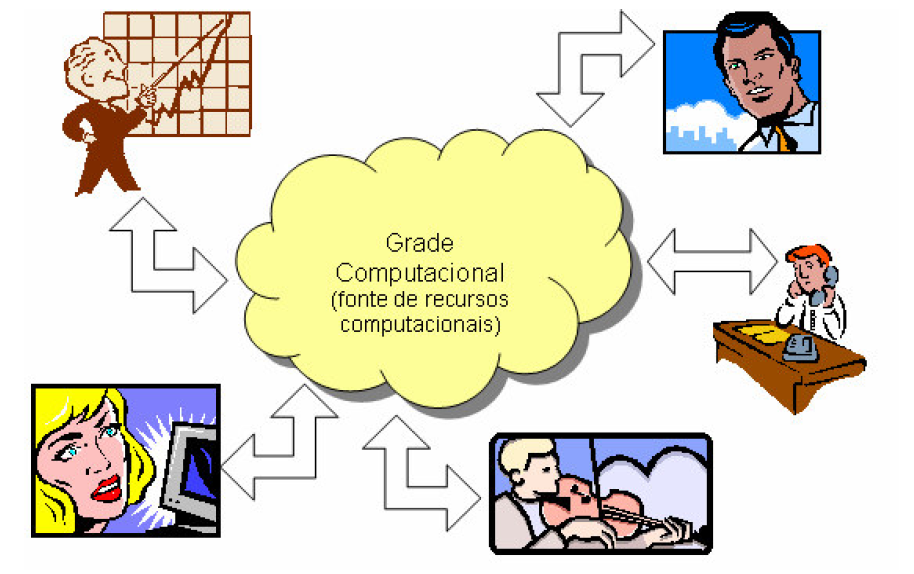
\includegraphics[width=0.6\textwidth]{figuras/grade-comp.png}
	% Caption centralizada
% 	\captionsetup{justification=centering}
	% Caption e fonte 
	 \vspace{-0.2cm}
	\\\textbf{\footnotesize Fonte: \cite{cap-livro} }
	\label{fig:figura1}
\end{figure}
\vspace{-0.5cm}

\subsection{\esp Inserção de tela de software}

Nos casos de telas de \textit{software}, devem ser inseridas como figuras, e referenciadas no texto
como na Figura \ref{fig:tela1}. Além disso, é necessário que seja citada no texto a empresa desenvolvedora.

% Figura
\begin{figure}[!ht]
	\centering	
	\caption[\hspace{0.1cm}Exemplo de tela de software.]{Exemplo de tela de software}
	  \vspace{-0.4cm}
	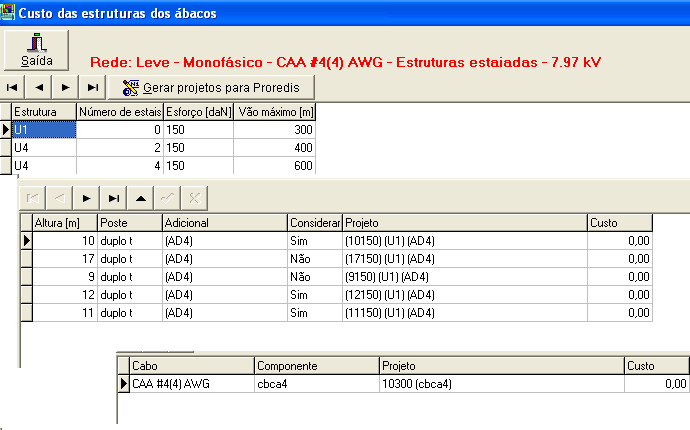
\includegraphics[width=.8\textwidth]{figuras/tela1.png}
	% Caption centralizada
% 	\captionsetup{justification=centering}
	% Caption e fonte
	 \vspace{-0.3cm}
	\\\textbf{\footnotesize Fonte: \cite{tela1}}
	\label{fig:tela1}
\end{figure}

\subsection{\esp Inserção de gráficos e mapas}

O gráfico é um tipo de ilustração que deve conter todos os elementos citados e também a descrição de seu título
diferenciando-o das figuras da mesma forma que no Gráfico 1. 

\begin{center}
	\centering	
 	\textbf{Gráfico 1 - Exemplo de um gráfico} \\
%  	  \vspace{0.cm}
	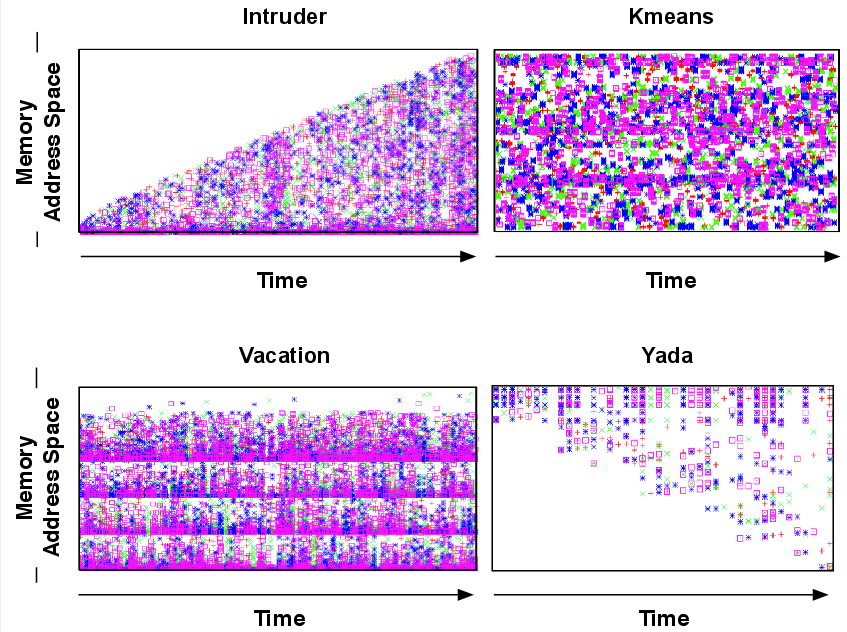
\includegraphics[width=0.7\textwidth]{figuras/access.png}
	% Caption centralizada
% 	\captionsetup{justification=centering}
	% Caption e fonte
	 \vspace{-0.3cm}
	\\\textbf{\footnotesize Fonte: \cite{tese}}
	\label{grafico1}
\end{center}

A mesma regra se aplica para mapas, que devem ser adicionados seguindo as regras de apresentação já mostradas. No caso específico,
o título e a numeração, também como os gráficos, devem começar do numeral ``1'' depois da marcação ``Mapa'' seguido do nome do elemento.
Exemplo: \textbf{Mapa 1 - Exemplo de um Mapa}.

 \subsection{\esp Tabelas}

As tabelas devem ser abertas nas laterais, com espaços verticais separando
as colunas e sem espaços horizontais, exceto na
separação do cabeçalho. Um exemplo é a Tabela \ref{tab:tabela1}. 

% Tabela
\begin{table}[htb]
	\centering
	\caption{\hspace{0.1cm} Exemplo de uma tabela}
	\vspace{-0.3cm} % espaço entre titulo e tabela
	\label{tab:tabela1}
	% Conteúdo da tabela
	\begin{tabular}{l|c|c}
  \hline
    \textbf{Imagem}	& \textbf{transferência} & \textbf{tempo} \\
    \hline
     estação 1	& 7,72 MB/s &  1:22:18 \\
     estação 2	& 7,72 MB/s &  1:22:17 \\
     estação 3	& 7,59 MB/s & 1:24:25 \\
     estação 4  & 7,53 MB/s & 1:43:27 \\
     estação 5	& 6,14 MB/s  &  1:24:41 \\
     estação 6  &  7,50 MB/s & 1:23:53 \\
     estação 7  & 7,58 MB/s  &  1:24:02 \\
     estação 8  & 7,8 MB/s  &  1:29:06 \\
     estação 9  & 7,9 MB/s  &  1:30:05 \\
     estação 10 & 8,0 MB/s  &  1:32:03 \\
     \hline
 \end{tabular}
 	\vspace{.1cm}  %espaço entre tabela e fonte
	\small
	% Fonte
	{\footnotesize\\ \textbf{Fonte: \cite{monog-fabio}}}
\end{table}

\subsection{\esp Quadros}

Os quadros diferem das tabelas por apresentarem dados textuais.
Esses dados podem ser esquemáticos, comparativos ou descritivos.

   \begin{center}
          \centering
       	\textbf{Quadro 1 - Bandas/Artistas de Rock e outros}\\
% 	\vspace{-0.3cm} % espaço entre titulo e tabela
        \label{quadro1}
	\begin{tabular}{|c|c|c|c|} \hline
	\multicolumn{4}{|c|}{\textbf{Bandas ou Artigas de Rock e outros}} 	  \\ 
		\hline \textbf{	Progressivo} & Pink Floyd & Jethro Tull	& Yesterday \\ 
		 \hline \textbf{ Metal}  & Metallica & Iron Maidam & Black Sabath \\ 
		\hline \textbf{	Arena Rock} & Led Zeppelin & The Rolling Stones & Beatles \\ 
		\hline \textbf{ Punk} & Ramones & Black Flag & NOFX	\\ 
		\hline \textbf{	Nacional} & Ira & Engenheiros & Vinil	\\ 
		\hline \textbf{	S.J.E.} & Apolo XI & Invasão 7 & Por do Sol \\ 
		\hline \textbf{	Grunge} & Nirvana & Pear Jam & Alice in Chains	\\ 
		\hline \textbf{	Rock Folk} & Bod Dylan & The Byrds &  The Mamas \& the Papas \\
		\hline \textbf{	Blues} & B.B. King & Albert Colins & Mady Wathers \\ 
		\hline \textbf{	New Wave} & The Police & The Pretenders, &  Duran Duran\\ 
 		\hline \textbf{	Rock Folk} & Bod Dylan & The Byrds &  The Mamas \& the Papas \\
 		\hline \textbf{	Rock alternativo} & R.E.M.& Hüsker Dü & Big Black\\ 
 		
		\hline
	\end{tabular}
	\vspace{0.1cm} 
	{\footnotesize\\ \textbf{Fonte: Dados da pesquisa}}
   \end{center}

Para gráficos, quadros e tabelas, cujos dados foram extraídos da própria pesquisa, 
 usar a expressão: Dados da pesquisa. Ver exemplo no Quadro 1.
   

\subsection{\esp Inserção de algoritmos}

Para inserir um algoritmo, utilizar o exemplo do Algoritmo  \ref{alg:rnagenerica}.
Todos os algoritmos devem ser inseridos como figura, indicada por nome e  fonte. Caso 
forem de própria autoria, isso deverá ser mencionado na fonte, como elaboração feita pelos autores.

% algoritmo
% \begin{figure}[ht]
\begin{center}	
	% Arquivo da figura
% 	\caption[\hspace{0.1cm} Texto da figuras.]{Algorítmo CAC RD Neural}
         \textbf{Algoritmo 1 -  CAC RD Neural}
	\vspace{-0.3cm}
\begin{minipage}[ht]{13cm}
\begin{algorithm}[H]
  \footnotesize
  \caption{CAC-RD Neural}
  \label{alg:rnagenerica}
  \begin{algorithmic}[1]
      \STATE \textbf{Entrada:} Requisição da chamada
    \STATE \textbf{Saída:} Aceitação ou bloqueio da solicitação
    
    \STATE Preenche o vetor de $attributes.size+1$ atributos com os valores dos atributos, sendo a primeira posição do vetor preenchida com o valor 1
		\STATE $hidden\_layer\_size =  attributes.size*2+1;$

    \FOR{$i$ = 1 to $attributes.size+1$}
    	\STATE \textbf{normalizar}($Entrada_i$)
    \ENDFOR

		\STATE $double [] net = new double [hidden\_layer\_size];$
    \STATE $net = hidden\_layer\_weights * attributes;$
   	\FOR{$i$ = 0 to hidden\_layer\_size}
			\STATE $net [i] = 1.0 / (1.0 + exp((-1.0)*net[i]));$
		\ENDFOR

		\STATE $double [] ipVector = new double [hidden\_layer\_size+1];$
    \STATE $ipVector [0] = 1.0;$
   	\FOR{$i$ = 1 to $hidden\_layer\_size+1$}
			\STATE $ipVector [i] = net [i-1];$
		\ENDFOR
		
		\STATE $output = output\_layer\_weights *  ipVector;$
    \STATE output = \textbf{desnormalizar}(Saída)
    \STATE \textbf{net\_update} (requisition);
    
    \STATE \textbf{Retorna} output; FIM
  \end{algorithmic}
\end{algorithm}
% \vspace{-0.3cm} % espaço entre algoritmo e fonte

\small \centering \textbf{\footnotesize Fonte: \cite{mestrado}.}
\end{minipage}
\end{center}
% \end{figure}

Para ilustrações criadas ou adaptadas a partir de outras ilustrações, usar as expressões: 
“Adaptado de...” ou “Criado pelo autor`` com dados extraídos de \ldots
   
   
\section{\esp CITAÇÕES}


Referências deverão ser adicionadas no arquivo \textit{bibliografia.bib}. Cada referência deverá ser adicionada conforme o padrão de normalização da PUC, 
o qual poderá ser consultado na página da biblioteca da PUC Minas \cite{manualpuc}. Todas as publicações citadas no texto deverão ter correspondente nas referências, 
e as indicações de autoria da citação e do ano deverão ser idênticas aos dados expostos.


\subsection{\esp Citação livre ou indireta}

Quando se reproduzir ideias, sem transcrever as palavras do autor, a indicação da página é opcional. Exemplos desse tipo de citação:
\begin{enumerate} 
 \item [a)] Citação com um autor \cite{knuth}. 
 \item [b)] Citação de artigos em revistas com dois autores \cite{artigo01}.
  \item [c)] Trabalho em congresso com três autores \cite{dovzan:01}.
 \item [d)] Trabalhos com mais de três autores \cite{cap-livro}.
 \item [e)] Dois autores em duas obras distintas \cite{knuth,groupp}.
 \item [d)] Trabalhos distintos com vários autores \cite{congresso,cap-livro}.
 
\end{enumerate}

\subsection{\esp Citação direta ou textual}

Transcrição literal de textos de outros autores. Nesse caso, deverão ser especificadas as páginas consultadas. 
Se desejar, poderão ser grafadas em itálico para melhor visualização.

\subsubsection{\esp Textual Curtas}

Quando curtas (até 3 linhas) serão inseridas na sequência normal do texto, entre aspas com as mesma formatação.

\subsubsection{\esp Textual Longas}

Citações longas (mais de 3 linhas) deverão constituir um parágrafo independente, recuado a 4 cm da margem esquerda, 
com letra tamanho 10 e digitado em espaço simples, sem aspas.
\begin{citacaodireta}
Hegel chama trabalho à forma específica da satisfação das necessidades, que
distingue da natureza o espírito existente. Assim como a linguagem infringe
a imposição da intuição e ordena o caos das múltiplas sensações em coisas
identificáveis, assim o trabalho infringe a imposição do \hspace{0.1cm}desejo \hspace{0.1cm}imediato \hspace{0.1cm}e
suspende, por assim dizer, o processo de satisfação das necessidades.
\cite[25]{habermas}.
\end{citacaodireta}


% Artigo \cite{whatershed:01}

\subsubsection{\esp Textual de outros idiomas (Tradução)}

\begin{citacaodireta} 
Um \textit{cluster} é um computador paralelo construído de componentes e processos de \textit{software} (tal como sistema de \textit{software}). 
Um \textit{cluster} é formado de nós, cada um contendo um ou mais processadores, memória que é compartilhada por todos os processadores do nodo 
(somente eles), e dispositivos periféricos adicionais (tais como discos), conectados pela rede e que permitem tráfego de dados entre os nós...
\cite[p. 10, tradução nossa]{groupp}\footnote {  … a cluster is a parallel computer that is constructed of commodity  componets and runs 
(as its system software) commodity software. A cluster is made of nodes, each conteining one or more processors, memory that is  shared 
by all of the processors in (and only on) the node, and addtional peripheral devices (surch as disks),
 connected by network that allows data to move between the nodes}.
\end{citacaodireta}
 
\subsection{\esp Exemplos de citações} 

Alguns exemplos de citações mais utilizadas e/ou que geram algumas dúvidas. É válido observar que não citaremos
todas as possibilidades de citações da norma da PUC Minas, sendo assim é de extrema relevância que se consulte 
o documento no site da Biblioteca da PUC Minas para maiores esclarecimentos acerca de citações \cite{manualpuc}.

\subsubsection{\esp Citação de monografia, dissertação e tese}

Exemplo de citação de monografia de curso de graduação ou especialização pode ser vista em \citeonline{monog-fabio}.
Exemplo de dissertação de mestrado é referida como \citeonline{mestrado}.

Para o caso de doutorado é citado da seguinte forma, Góes (\citeyear{tese}). Nesse exemplo é válido observar a forma
como está escrito no documento \LaTeX, pois citações que compreendem no texto o nome do autor como sua parte, necessitam 
do parâmetro \verb$\citeonline{}$. 

\subsubsection{\esp Livros e partes de livros}

Exemplo de capítulo de livro fica conforme este exemplo \cite{cap-livro}.

Para livros citados no corpo do texto e com duas citações juntas, ver os exemplos \citeonline{knuth,groupp}.
Caso essa citação não fizesse parte do texto será referencia dessa forma \cite{knuth,groupp}.

Citações institucionais ou documentos técnicos de alguma entidade devem ser citados desta forma \cite{pmbok}.

\subsubsection{\esp Tela de software}

Para  citar a tela de um \textit{software} faça da seguinte forma, \citeonline{tela1}.

\subsubsection{\esp Citações da Biblia Sagrada}

A Bíblia está dividida em duas grandes partes: O Antigo Testamento e o Novo Testamento, divididos em livros, capítulos e versículos. 
Portanto, a citação de partes da Bíblia deve apresentar o título do livro de forma abreviada ou por extenso, o número do capítulo e o número do versículo.


\begin{citacaodireta}
Moisés estendeu a mão sobre o mar. Com um forte \hspace{-0.1cm} vento \hspace{0.1cm} leste a \hspace{0.1cm}sobrar a
noite toda, o Senhor repeliu o mar e o pôs a seco. As águas se fenderam e
os filhos de Israel entraram no meio do mar a pé enxuto, enquanto as águas
formavam uma muralha à direita e à esquerda deles (\citeauthor{biblia} 14,21).
\end{citacaodireta}

\subsection{\esp Conclusão}

Discussão dos resultados obtidos na pesquisa. É onde se colocam as observações do autor. 
Poderá também apresentar sugestões de novas linhas de estudo.

A conclusão deve estar de acordo com os objetivos do trabalho.

A conclusão não deve apresentar citações ou interpretações de outros autores.

% \subsection{\esp Trabalhos futuros}
% 
% Sugestões de estudos posteriores são ser adicionados subseção deste capítulo de conclusão.

%%%%%%%%%%%%%%%%%%%%%%%%%%%%%%%%%%%
%% FIM DO TEXTO
%%%%%%%%%%%%%%%%%%%%%%%%%%%%%%%%%%%

% \selectlanguage{brazil}
%%%%%%%%%%%%%%%%%%%%%%%%%%%%%%%%%%%
%% Inicio bibliografia
%%%%%%%%%%%%%%%%%%%%%%%%%%%%%%%%%%%

 \newpage
 \singlespace{
 \bibliographystyle{abntex2-alf}
 \bibliography{bibliografia}
 }

\end{document}